\documentclass[]{article}
\usepackage[T1]{fontenc}
\usepackage{lmodern}
\usepackage{amssymb,amsmath}
\usepackage{ifxetex,ifluatex}
\usepackage{fixltx2e} % provides \textsubscript
% use upquote if available, for straight quotes in verbatim environments
\IfFileExists{upquote.sty}{\usepackage{upquote}}{}
\ifnum 0\ifxetex 1\fi\ifluatex 1\fi=0 % if pdftex
  \usepackage[utf8]{inputenc}
\else % if luatex or xelatex
  \ifxetex
    \usepackage{mathspec}
    \usepackage{xltxtra,xunicode}
  \else
    \usepackage{fontspec}
  \fi
  \defaultfontfeatures{Mapping=tex-text,Scale=MatchLowercase}
  \newcommand{\euro}{€}
\fi
% use microtype if available
\IfFileExists{microtype.sty}{\usepackage{microtype}}{}
\usepackage{longtable,booktabs}
\usepackage{graphicx}
% Redefine \includegraphics so that, unless explicit options are
% given, the image width will not exceed the width of the page.
% Images get their normal width if they fit onto the page, but
% are scaled down if they would overflow the margins.
\makeatletter
\def\ScaleIfNeeded{%
  \ifdim\Gin@nat@width>\linewidth
    \linewidth
  \else
    \Gin@nat@width
  \fi
}
\makeatother
\let\Oldincludegraphics\includegraphics
{%
 \catcode`\@=11\relax%
 \gdef\includegraphics{\@ifnextchar[{\Oldincludegraphics}{\Oldincludegraphics[width=\ScaleIfNeeded]}}%
}%
\ifxetex
  \usepackage[setpagesize=false, % page size defined by xetex
              unicode=false, % unicode breaks when used with xetex
              xetex]{hyperref}
\else
  \usepackage[unicode=true]{hyperref}
\fi
\hypersetup{breaklinks=true,
            bookmarks=true,
            pdfauthor={Daniel Bruder},
            pdftitle={ppp Documentation},
            colorlinks=true,
            citecolor=blue,
            urlcolor=blue,
            linkcolor=magenta,
            pdfborder={0 0 0}}
\urlstyle{same}  % don't use monospace font for urls
\setlength{\parindent}{0pt}
\setlength{\parskip}{6pt plus 2pt minus 1pt}
\setlength{\emergencystretch}{3em}  % prevent overfull lines
\setcounter{secnumdepth}{5}

\title{\texttt{ppp} Documentation}
\author{Daniel Bruder}
\date{Version 0.9.0}

\begin{document}
\maketitle

\newpage

\section{Abstract}\label{abstract}

\emph{\texttt{ppp} allows you to use pandoc in new ways by rendering
ASCII-markup to beautiful pictures right from within pandoc's verbatim
environments.}

\emph{See below for illustrative examples and detailed usage
instructions.}

\emph{Bonus on top: Leaving out \texttt{ppp} form the typesetting
pipeline will still render your document and the verbatims with the
ASCII-markup will still stay readable!}

\begin{center}\rule{3in}{0.4pt}\end{center}

\newpage
\tableofcontents
\newpage

\section{General usage}\label{general-usage}

In each case, you will use pandoc's verbatim environment, set the
rendering engine and additional options:

\begin{verbatim}
~~~~~ {.renderer .option1 .option2=value2}
 --- RENDERER-SPECIFIC MARKUP GOES HERE ---
~~~~~
\end{verbatim}

\subsection{General Renderers}\label{general-renderers}

The renderers available to \texttt{ppp} are:

\begin{itemize}
\itemsep1pt\parskip0pt\parsep0pt
\item
  ditaa
\item
  yuml diagrams:

  \begin{itemize}
  \itemsep1pt\parskip0pt\parsep0pt
  \item
    class diagramas (cf.~Figure \ref{fig:yuml-class-diagram})
  \item
    usecase diagramas (cf.~Figure \ref{fig:yuml-usecase-diagram})
  \item
    activity diagramas (cf.~Figure \ref{fig:yuml-activity-diagram})
  \end{itemize}
\item
  dot
\item
  neato
\item
  rdfdot
\item
  plantuml
\end{itemize}

\hyperdef{}{general-options}{\subsection{General
Options}\label{general-options}}

This is a list of the general options, compatible with any type of
renderer:

\begin{itemize}
\itemsep1pt\parskip0pt\parsep0pt
\item
  \texttt{.scale=90\%}
\item
  \texttt{.label=fig:my-figure}
\item
  \texttt{.title="Some label for the figure"}
\end{itemize}

\begin{center}\rule{3in}{0.4pt}\end{center}

\newpage

\section{ditaa Diagrams}\label{ditaa-diagrams}

In order to generate \texttt{ditaa}-diagrams, ditaa needs to be
installed.

For an exhaustive list of options and possibilities, please check the
\href{http://ditaa.sourceforge.net/}{ditaa homepage}.

\subsection{ditaa Options}\label{ditaa-options}

Apart from the \hyperref[general-options]{General Options}, the possible
options specific to ditaa are:

\begin{itemize}
\itemsep1pt\parskip0pt\parsep0pt
\item
  \texttt{.rounded-corners}
\item
  \texttt{.no-shadows}
\item
  \texttt{.no-antialias}
\item
  \texttt{.no-separation}
\end{itemize}

\subsection{ditaa Examples}\label{ditaa-examples}

Using ditaa, the following markup will produce Figure
\ref{fig:pipeline-overview}.

\scriptsize

\begin{verbatim}
~~~~~ {.ditaa .rounded-corners .no-shadows .scale=90%
       .title="The ppp and pandoc pipeline"
       .label=fig:pipeline-overview 
       .no-antialias .no-separation}
# Caution! These lines actually would have to be on *one* line only!
+-----------------+       +--------+           +--------------------+
| markdown source |------>| ppp    |------*--->| pröcessed markdown |
+-----------------+       +--------+      |    +--------------------+
                              |           \--->| image files        |
                    +------------------+       +--------------------+
                    | diagram creation |
                    +------------------+
                    | ditaa/dot/rdfdot |
                    +------------------+
~~~~~
\end{verbatim}

\normalsize

\begin{figure}[htbp]
\centering
\includegraphics{/Users/dbruder/tmp/FQdjc5eyxZ/image-1.png}
\caption{``The ppp and pandoc pipeline''\label{fig:pipeline-overview-x}}
\end{figure}

\begin{figure}[htbp]
\centering
\includegraphics{/Users/dbruder/tmp/FQdjc5eyxZ/image-2.png}
\caption{``The ppp and pandoc pipeline''\label{fig:pipeline-overview-y}}
\end{figure}

As a contrast, turning off several options, ditaa will produce an output
as in Figure \ref{fig:pipeline-overview-2}:

\scriptsize

\begin{verbatim}
~~~~~ {.ditaa .scale=90% .title="The ppp and pandoc pipeline #2" .label=fig:pipeline-overview-2}
+-----------------+       +--------+           +--------------------+
| markdown source |------>| ppp    |------*--->| pröcessed markdown |
+-----------------+       +--------+      |    +--------------------+
                              |           \--->| image files        |
                    +------------------+       +--------------------+
                    | diagram creation |
                    +------------------+
                    | ditaa/dot/rdfdot |
                    +------------------+
~~~~~
\end{verbatim}

\normalsize

\begin{figure}[htbp]
\centering
\includegraphics{/Users/dbruder/tmp/FQdjc5eyxZ/image-3.png}
\caption{``The ppp and pandoc pipeline
\#2''\label{fig:pipeline-overview-2}}
\end{figure}

\begin{center}\rule{3in}{0.4pt}\end{center}

\newpage

\hyperdef{}{dot-diagrams}{\section{dot Diagrams}\label{dot-diagrams}}

\texttt{dot} rendering is done through
\href{http://www.graphviz.org/}{GraphViz}'s engine. Please cf.
\href{http://www.graphviz.org/Documentation.php}{Graphviz's
Documentation} for exact usage specifics on the usage of \texttt{dot}.

\hyperdef{}{dot-options}{\subsection{dot Options}\label{dot-options}}

\begin{itemize}
\itemsep1pt\parskip0pt\parsep0pt
\item
  currently none apart from the \hyperref[general-options]{General
  Options}
\end{itemize}

\subsection{dot Examples}\label{dot-examples}

With \texttt{dot} as the \emph{renderer}, the following markup produces
the figure as seen in Figure \ref{fig:dot-fsa}.

\scriptsize

\begin{verbatim}
~~~~~ {.dot .scale=50% .title=dot Finite State Automaton .label=fig:dot-fsa}
digraph finite_state_machine {
  rankdir=LR;
  node [shape = doublecircle]; LR_0 LR_3 LR_4 LR_8;
  node [shape = circle];
  LR_0 -> LR_2 [ label = "SS(B)" ];
  LR_0 -> LR_1 [ label = "SS(S)" ];
  LR_1 -> LR_3 [ label = "S($end)" ];
  LR_2 -> LR_6 [ label = "SS(b)" ];
  LR_2 -> LR_5 [ label = "SS(a)" ];
  LR_2 -> LR_4 [ label = "S(A)" ];
  LR_5 -> LR_7 [ label = "S(b)" ];
  LR_5 -> LR_5 [ label = "S(a)" ];
  LR_6 -> LR_6 [ label = "S(b)" ];
  LR_6 -> LR_5 [ label = "S(a)" ];
  LR_7 -> LR_8 [ label = "S(b)" ];
  LR_7 -> LR_5 [ label = "S(a)" ];
  LR_8 -> LR_6 [ label = "S(b)" ];
  LR_8 -> LR_5 [ label = "S(a)" ];
}
~~~~~
\end{verbatim}

\normalsize

\begin{figure}[htbp]
\centering
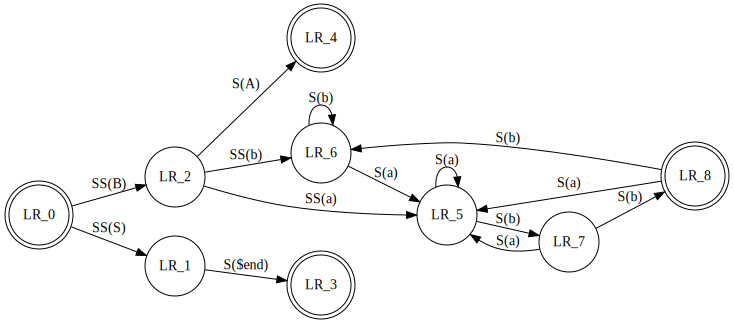
\includegraphics{/Users/dbruder/tmp/FQdjc5eyxZ/image-4.png}
\caption{dot Finite State Automaton\label{fig:dot-fsa}}
\end{figure}

\begin{center}\rule{3in}{0.4pt}\end{center}

\newpage

\section{neato Diagrams}\label{neato-diagrams}

\texttt{neato} diagrams behave very similarly to
\hyperref[dot-diagrams]{dot Diagrams}. Please cf
\hyperref[dot-diagrams]{dot Diagrams} for more information

\subsection{neato Options}\label{neato-options}

\begin{itemize}
\itemsep1pt\parskip0pt\parsep0pt
\item
  same as \hyperref[dot-options]{dot Options}
\end{itemize}

\subsection{neato Examples}\label{neato-examples}

The following example produces Figure \ref{fig:neato-diagram}.

\scriptsize

\begin{verbatim}
~~~~~ {.neato .scale=80% .title=neato diagram .label=fig:neato-diagram}
graph G {
  n0 -- n1 -- n2 -- n3 -- n0;
}
~~~~~
\end{verbatim}

\normalsize

\begin{figure}[htbp]
\centering
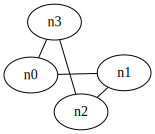
\includegraphics{/Users/dbruder/tmp/FQdjc5eyxZ/image-5.png}
\caption{neato diagram\label{fig:neato-diagram}}
\end{figure}

\begin{center}\rule{3in}{0.4pt}\end{center}

\newpage

\section{yUML}\label{yuml}

yUML needs a network connection and uses http://yuml.me as the rendering
service.

\subsection{yUML Options}\label{yuml-options}

Options specific to yUML can be:

\begin{itemize}
\itemsep1pt\parskip0pt\parsep0pt
\item
  \texttt{.type=}: any of \texttt{{[}} \texttt{class},
  \texttt{activity}, \texttt{usecase} \texttt{{]}}
\item
  \texttt{.style=}: any of \texttt{{[}} \texttt{scruffy},
  \texttt{nofunky}, \texttt{plain} \texttt{{]}}
\item
  \texttt{.direction=}: any of \texttt{{[}} \texttt{LR}, \texttt{RL},
  \texttt{TD}, \texttt{{]}}
\end{itemize}

\subsection{yUML Examples}\label{yuml-examples}

\subsubsection{yUML Class diagrams}\label{yuml-class-diagrams}

With \emph{yUML} as the renderer, setting \texttt{.type=class} and using
the style \texttt{.style=nofunky}, the following markup produces Figure
\ref{fig:yuml-class-diagram}.

\scriptsize

\begin{verbatim}
~~~~ {.yuml .style=nofunky .type=class .direction=LR .scale=100% .title=yUML class diagram .label=fig:yuml-class-diagram}
[Customer] +1 ->        *[Order]
[Order]   ++1 -items>   *[LineItem]
[Order]       -0..1>     [PaymentMethod]
~~~~
\end{verbatim}

\normalsize

\begin{figure}[htbp]
\centering
\includegraphics{/Users/dbruder/tmp/FQdjc5eyxZ/image-6.png}
\caption{yUML class diagram\label{fig:yuml-class-diagram}}
\end{figure}

\newpage

\subsubsection{yuml Usecase diagrams}\label{yuml-usecase-diagrams}

With \texttt{scruffy} style and \texttt{.type=usecase}, the following
example produces Figure \ref{fig:yuml-usecase-diagram}.

\scriptsize

\begin{verbatim}
~~~~ {.yuml .style=scruffy .type=usecase .title=yUML usecase diagram .label=fig:yuml-usecase-diagram}
// Cool Use Case Diagram
[Customer]-(Make Cup of Tea)
(Make Cup of Tea)<(Add Milk)
(Make Cup of Tea)>(Add Tea Bag)
~~~~
\end{verbatim}

\normalsize

\begin{figure}[htbp]
\centering
\includegraphics{/Users/dbruder/tmp/FQdjc5eyxZ/image-7.png}
\caption{yUML usecase diagram\label{fig:yuml-usecase-diagram}}
\end{figure}

\newpage

\subsubsection{yuml Activity diagrams}\label{yuml-activity-diagrams}

Lastly, using \texttt{.type=activity} and \texttt{.style=plain} the
following example produces Figure \ref{fig:yuml-activity-diagram}.

\scriptsize

\begin{verbatim}
~~~~ {.yuml .style=plain .type=activity .title=yUML activity Diagram .label=fig:yuml-activity-diagram}
(start)->|a|,|a|->(Make Coffee)->|b|,|a|->(Make Breakfast)->|b|,|b|-><c>[want more coffee]->(Make Coffee),<c>[satisfied]->(end)
~~~~
\end{verbatim}

\normalsize

\begin{figure}[htbp]
\centering
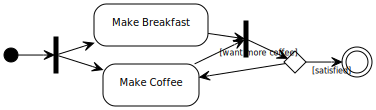
\includegraphics{/Users/dbruder/tmp/FQdjc5eyxZ/image-8.png}
\caption{yUML activity Diagram\label{fig:yuml-activity-diagram}}
\end{figure}

\begin{center}\rule{3in}{0.4pt}\end{center}

\newpage

\section{plantuml}\label{plantuml}

plantuml -- based on graphviz --, has an extensive feature set

\subsection{plantuml Options}\label{plantuml-options}

\begin{itemize}
\itemsep1pt\parskip0pt\parsep0pt
\item
  \emph{General Options}
\end{itemize}

\subsection{plantuml Examples}\label{plantuml-examples}

\subsubsection{plantuml Example 1}\label{plantuml-example-1}

With \emph{plantuml} as the renderer, the following markup produces
Figure \ref{fig:plantuml-example-1}.

\scriptsize

\begin{verbatim}
~~~~ {.plantuml .scale=60% .title=PlantUML Example 1 .label=fig:plantuml-example-1}
@startuml
scale 350 width
[*] --> NotShooting

state NotShooting {
  [*] --> Idle
  Idle --> Configuring : EvConfig
  Configuring --> Idle : EvConfig
}

state Configuring {
  [*] --> NewValueSelection
  NewValueSelection --> NewValuePreview : EvNewValue
  NewValuePreview --> NewValueSelection : EvNewValueRejected
  NewValuePreview --> NewValueSelection : EvNewValueSaved

  state NewValuePreview {
     State1 -> State2
  }

}
@enduml
~~~~
\end{verbatim}

\normalsize

\begin{figure}[htbp]
\centering
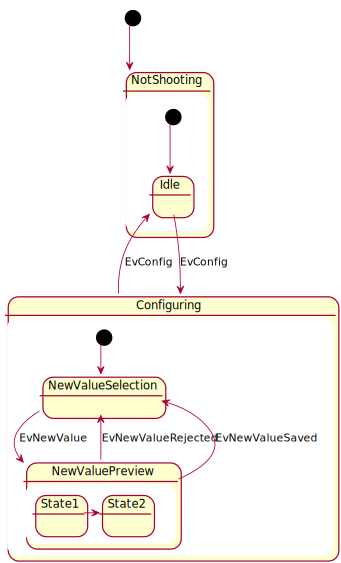
\includegraphics{/Users/dbruder/tmp/FQdjc5eyxZ/image-9.png}
\caption{PlantUML Example 1\label{fig:plantuml-example-1}}
\end{figure}

\newpage

\subsubsection{plantuml Example 2}\label{plantuml-example-2}

If the colors don't match your taste exactly, add
\texttt{skinparam monochrome true} to retrieve Figure
\ref{fig:plantuml-example-2}.

\scriptsize

\begin{verbatim}
~~~~ {.plantuml .scale=120% .title=PlantUML Example 2 .label=fig:plantuml-example-2}
@startuml

skinparam monochrome true

actor User
participant "First Class" as A
participant "Second Class" as B
participant "Last Class" as C

User -> A: DoWork
activate A

A -> B: Create Request
activate B

B -> C: DoWork
activate C
C --> B: WorkDone
destroy C

B --> A: Request Created
deactivate B

A --> User: Done
deactivate A

@enduml
~~~~
\end{verbatim}

\normalsize

\begin{figure}[htbp]
\centering
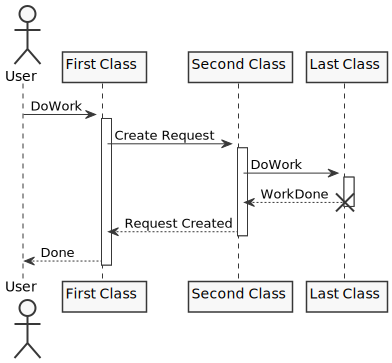
\includegraphics{/Users/dbruder/tmp/FQdjc5eyxZ/image-10.png}
\caption{PlantUML Example 2\label{fig:plantuml-example-2}}
\end{figure}

\newpage

\begin{center}\rule{3in}{0.4pt}\end{center}

\newpage

\section{rdfdot Diagrams}\label{rdfdot-diagrams}

\subsection{rdfdot Options}\label{rdfdot-options}

\begin{itemize}
\itemsep1pt\parskip0pt\parsep0pt
\item
  currently none apart from the \hyperref[general-options]{General
  Options}
\end{itemize}

\subsection{rdfdot Examples}\label{rdfdot-examples}

The following example produces Figure \ref{"fig:rdfdot-diagram"} on page
\pageref{"fig:rdfdot-diagram"}.

\scriptsize

\begin{verbatim}
~~~~~ {.rdfdot .scale=150% .title=rdfdot Diagram .label="fig:rdfdot-diagram"}
@prefix foaf: <http://xmlns.com/foaf/0.1/> .
@base <http://example.com/> .
<alice> foaf:name "Alice" ;
        foaf:knows [ foaf:name "Bob" ] .
~~~~~
\end{verbatim}

\normalsize

\begin{figure}[htbp]
\centering
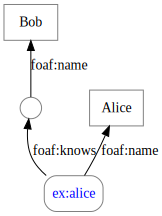
\includegraphics{/Users/dbruder/tmp/FQdjc5eyxZ/image-11.png}
\caption{rdfdot Diagram\label{"fig:rdfdot-diagram"}}
\end{figure}

\newpage

\section{List of options}\label{list-of-options}

\begin{longtable}[c]{@{}ccc@{}}
\toprule\addlinespace
\begin{minipage}[b]{0.28\columnwidth}\centering
Renderer
\end{minipage} & \begin{minipage}[b]{0.33\columnwidth}\centering
Option
\end{minipage} & \begin{minipage}[b]{0.25\columnwidth}\centering
possible values
\end{minipage}
\\\addlinespace
\midrule\endhead
\begin{minipage}[t]{0.28\columnwidth}\centering
\emph{General}
\end{minipage} & \begin{minipage}[t]{0.33\columnwidth}\centering
\texttt{.scale}
\end{minipage} & \begin{minipage}[t]{0.25\columnwidth}\centering
e.g. \texttt{120\%}
\end{minipage}
\\\addlinespace
\begin{minipage}[t]{0.28\columnwidth}\centering
\end{minipage} & \begin{minipage}[t]{0.33\columnwidth}\centering
\texttt{.label}
\end{minipage} & \begin{minipage}[t]{0.25\columnwidth}\centering
\texttt{fig:my-figure}
\end{minipage}
\\\addlinespace
\begin{minipage}[t]{0.28\columnwidth}\centering
\end{minipage} & \begin{minipage}[t]{0.33\columnwidth}\centering
\texttt{.title}
\end{minipage} & \begin{minipage}[t]{0.25\columnwidth}\centering
\texttt{"Some label for the figure"}
\end{minipage}
\\\addlinespace
\begin{minipage}[t]{0.28\columnwidth}\centering
ditaa
\end{minipage} & \begin{minipage}[t]{0.33\columnwidth}\centering
\texttt{.rounded-corners}
\end{minipage} & \begin{minipage}[t]{0.25\columnwidth}\centering
\end{minipage}
\\\addlinespace
\begin{minipage}[t]{0.28\columnwidth}\centering
\end{minipage} & \begin{minipage}[t]{0.33\columnwidth}\centering
\texttt{.no-shadows}
\end{minipage} & \begin{minipage}[t]{0.25\columnwidth}\centering
\end{minipage}
\\\addlinespace
\begin{minipage}[t]{0.28\columnwidth}\centering
\end{minipage} & \begin{minipage}[t]{0.33\columnwidth}\centering
\texttt{.no-antialias}
\end{minipage} & \begin{minipage}[t]{0.25\columnwidth}\centering
\end{minipage}
\\\addlinespace
\begin{minipage}[t]{0.28\columnwidth}\centering
\end{minipage} & \begin{minipage}[t]{0.33\columnwidth}\centering
\texttt{.no-separation}
\end{minipage} & \begin{minipage}[t]{0.25\columnwidth}\centering
\end{minipage}
\\\addlinespace
\begin{minipage}[t]{0.28\columnwidth}\centering
dot
\end{minipage} & \begin{minipage}[t]{0.33\columnwidth}\centering
N/A
\end{minipage} & \begin{minipage}[t]{0.25\columnwidth}\centering
\end{minipage}
\\\addlinespace
\begin{minipage}[t]{0.28\columnwidth}\centering
neato
\end{minipage} & \begin{minipage}[t]{0.33\columnwidth}\centering
N/A
\end{minipage} & \begin{minipage}[t]{0.25\columnwidth}\centering
\end{minipage}
\\\addlinespace
\begin{minipage}[t]{0.28\columnwidth}\centering
yUML
\end{minipage} & \begin{minipage}[t]{0.33\columnwidth}\centering
\texttt{.type=}
\end{minipage} & \begin{minipage}[t]{0.25\columnwidth}\centering
any of \texttt{{[}} \texttt{class}, \texttt{activity}, \texttt{usecase}
\texttt{{]}}
\end{minipage}
\\\addlinespace
\begin{minipage}[t]{0.28\columnwidth}\centering
\end{minipage} & \begin{minipage}[t]{0.33\columnwidth}\centering
\texttt{.style=}
\end{minipage} & \begin{minipage}[t]{0.25\columnwidth}\centering
any of \texttt{{[}} \texttt{scruffy}, \texttt{nofunky}, \texttt{plain}
\texttt{{]}}
\end{minipage}
\\\addlinespace
\begin{minipage}[t]{0.28\columnwidth}\centering
\end{minipage} & \begin{minipage}[t]{0.33\columnwidth}\centering
\texttt{.direction=}
\end{minipage} & \begin{minipage}[t]{0.25\columnwidth}\centering
any of \texttt{{[}} \texttt{LR}, \texttt{RL}, \texttt{TD}, \texttt{{]}}
\end{minipage}
\\\addlinespace
\begin{minipage}[t]{0.28\columnwidth}\centering
rdfdot
\end{minipage} & \begin{minipage}[t]{0.33\columnwidth}\centering
N/A
\end{minipage} & \begin{minipage}[t]{0.25\columnwidth}\centering
\end{minipage}
\\\addlinespace
\bottomrule
\addlinespace
\caption{List of options}
\end{longtable}

\newpage

\section{List of homepages and documentation to
renderers}\label{list-of-homepages-and-documentation-to-renderers}

\begin{longtable}[c]{@{}ll@{}}
\toprule\addlinespace
\begin{minipage}[b]{0.15\columnwidth}\raggedright
Renderer
\end{minipage} & \begin{minipage}[b]{0.79\columnwidth}\raggedright
Links
\end{minipage}
\\\addlinespace
\midrule\endhead
\begin{minipage}[t]{0.15\columnwidth}\raggedright
ppp
\end{minipage} & \begin{minipage}[t]{0.79\columnwidth}\raggedright
(this document)
\end{minipage}
\\\addlinespace
\begin{minipage}[t]{0.15\columnwidth}\raggedright
\end{minipage} & \begin{minipage}[t]{0.79\columnwidth}\raggedright
\url{https://metacpan.org/release/App-pandoc-preprocess}
\end{minipage}
\\\addlinespace
\begin{minipage}[t]{0.15\columnwidth}\raggedright
\end{minipage} & \begin{minipage}[t]{0.79\columnwidth}\raggedright
\url{https://github.com/xdbr/p5-App-pandoc-preprocess}
\end{minipage}
\\\addlinespace
\begin{minipage}[t]{0.15\columnwidth}\raggedright
ditaa
\end{minipage} & \begin{minipage}[t]{0.79\columnwidth}\raggedright
\url{http://ditaa.sourceforge.net/}
\end{minipage}
\\\addlinespace
\begin{minipage}[t]{0.15\columnwidth}\raggedright
dot
\end{minipage} & \begin{minipage}[t]{0.79\columnwidth}\raggedright
\url{http://www.graphviz.org/}
\end{minipage}
\\\addlinespace
\begin{minipage}[t]{0.15\columnwidth}\raggedright
neato
\end{minipage} & \begin{minipage}[t]{0.79\columnwidth}\raggedright
\url{http://www.graphviz.org/}
\end{minipage}
\\\addlinespace
\begin{minipage}[t]{0.15\columnwidth}\raggedright
yUML
\end{minipage} & \begin{minipage}[t]{0.79\columnwidth}\raggedright
\url{http://yuml.me/}
\end{minipage}
\\\addlinespace
\begin{minipage}[t]{0.15\columnwidth}\raggedright
\end{minipage} & \begin{minipage}[t]{0.79\columnwidth}\raggedright
\url{https://github.com/wandernauta/yuml}
\end{minipage}
\\\addlinespace
\begin{minipage}[t]{0.15\columnwidth}\raggedright
rdfdot
\end{minipage} & \begin{minipage}[t]{0.79\columnwidth}\raggedright
\url{https://metacpan.org/pod/RDF::Trine::Exporter::GraphViz}
\end{minipage}
\\\addlinespace
\begin{minipage}[t]{0.15\columnwidth}\raggedright
plantuml
\end{minipage} & \begin{minipage}[t]{0.79\columnwidth}\raggedright
\url{http://plantuml.sourceforge.net/}
\end{minipage}
\\\addlinespace
\bottomrule
\addlinespace
\caption{List of options}
\end{longtable}

\section{Credits and further
references}\label{credits-and-further-references}

\begin{itemize}
\itemsep1pt\parskip0pt\parsep0pt
\item
  \url{http://www.asciiflow.com/\#Draw}: an excellent helper for all
  things diagram
\item
  \url{http://randomdeterminism.wordpress.com/2012/06/01/how-i-stopped-worring-and-started-using-markdown-like-tex/}:
  general introduction to another approach to typesetting and using
  \texttt{gpp}
\item
  \url{https://github.com/nichtich/ditaa-markdown}: This is where the
  original idea came from
\item
  gpp: \url{http://files.nothingisreal.com/software/gpp/gpp.html}
\end{itemize}

\listoffigures

\begin{center}\rule{3in}{0.4pt}\end{center}

\end{document}
